\documentclass{article}

% if you need to pass options to natbib, use, e.g.:
% \PassOptionsToPackage{numbers, compress}{natbib}
% before loading nips_2016
%
% to avoid loading the natbib package, add option nonatbib:
% \usepackage[nonatbib]{nips_2016}

\usepackage{nips_2016}

% to compile a camera-ready version, add the [final] option, e.g.:
% \usepackage[final]{nips_2016}

\usepackage{color}
\usepackage[utf8]{inputenc} % allow utf-8 input
\usepackage[T1]{fontenc}    % use 8-bit T1 fonts
\usepackage{hyperref}       % hyperlinks
\usepackage{url}            % simple URL typesetting
\usepackage{booktabs}       % professional-quality tables
\usepackage{amsfonts}       % blackboard math symbols
\usepackage{nicefrac}       % compact symbols for 1/2, etc.
\usepackage{microtype}      % microtypography

\usepackage{url}
\usepackage{cleveref}
\usepackage[margin=0.3cm]{subcaption}
\usepackage{graphicx}
\usepackage{amsmath}
\usepackage{listings}
\usepackage{minted}

\newcommand{\N}{\mathcal{N}}
\newcommand{\E}{\mathbb{E}}
\newcommand{\G}{\mathfrak{G}}
\newcommand{\Tr}{\text{Tr}}
\renewcommand{\O}{\text{O}}
\newcommand{\diag}{\text{diag}}
\renewcommand{\v}[1]{\mathbf{#1}}
\newcommand{\I}{\v{I}}
\newcommand{\elbo}{{\sc elbo}}

\newcommand*\pFq[2]{{}_{#1}F_{#2}}%\genfrac[]{0pt}{}

\newcommand{\todo}[1]{{\color{red} \textbf{TODO:} {#1}}}

\title{Symmetrized Variational Inference}

% The \author macro works with any number of authors. There are two
% commands used to separate the names and addresses of multiple
% authors: \And and \AND.
%
% Using \And between authors leaves it to LaTeX to determine where to
% break the lines. Using \AND forces a line break at that point. So,
% if LaTeX puts 3 of 4 authors names on the first line, and the last
% on the second line, try using \AND instead of \And before the third
% author name.

\author{
  David A.~Moore\\
  Computer Science Division\\
  University of California, Berkeley\\
  \texttt{dmoore@cs.berkeley.edu} \\
}

\begin{document}
% \nipsfinalcopy is no longer used

\maketitle

\begin{abstract}
We introduce a framework for modeling parameter symmetries in
variational inference by explicitly mixing a base approximating density over a
symmetry group. We show that this can
be done tractably for the case of a Gaussian mixture over the
orthogonal group under an isotropic variance assumption. Initial results show that inference with
a symmetrized posterior avoids component collapse and leads to improved predictive performance. 
\end{abstract}

% highlevel TODOs:
% write introduction
% make nice visualization figure
% move messy stuff to supplement
% signflip experiments
% rotation experiments
% references

% the workshop paper can be whatever. but the story for an eventual
% long paper has to be intuitive. it has to be: there are real
% problems caused by the inability to capture the true posterior. it
% leads to worse predictive distributions. there is previous evidence
% both theoretical (implicit regularization) and empirical (bayesian
% PMF with MCMC) establishing this. 
%
% of course for a long paper there also has to be a plausible story
% for nonisotropic (and even non-uniform across rows) variances. and
% this goes hand in hand with VAEs and minibatch training. 
%
%
% related work:
%   - flexible approximating families (normalizing flows, stein, etc):
%   unless they have combinatorial power they will *all* be fucked up
%   by symmetries. a normalizing flow will waste its effort tracing
%   out O(n) rather than actually modeling the problem. Unless we
%   represent that structure *explicitly*. 
%
% mention: computing *correct* evidence bound incorporating
% symmetry. important for # of clusters. 
%
% to evaluate: 
%    - does ARD work for matrix factorization? 
%
%
\section{Introduction}

Many probability models commonly used in machine learning are not,
strictly speaking, identifiable: they exhibit {\em parameter
  symmetries} in which the model density is invariant under some class
of transformations of the latent parameters. The resulting multimodal posteriors
are not captured well by most inference procedures: ``label
switching'' is a well known problem in sampling mixture models \citep{neal1999erroneous,
  celeux2000computational}, while algorithms such as EP
that attempt to match marginals may miss crucial joint structure \citep{nishihara2013detecting}. 

It is sometimes thought that variational inference with a mode-seeking
divergence such as KL[$q\|p$] breaks symmetries by modeling only a
single mode of the posterior. However, symmetric modes are not isolated in latent space, but
in fact can bleed probability mass into each other to create new modes corresponding to degenerate
solutions. This ``implicit regularization'' results in approximate
inference failing to use a model's full representational capacity. This effect has been noted for
Gaussian mixture models \citep{mackay2001local} and analyzed
extensively in the case of matrix factorization
\citep{nakajima2010implicit,nakajima2013global}. An analogous phenomenon may be
observed in component collapse of variational autoencoders
\citep{dinh2014cifar, burda2015importance}. 

We propose modeling symmetries directly in variational inference using a {\em symmetrized
  posterior} formed by explicitly mixing a ``base'' 
distribution over the relevant symmetry group, so that our approximating
class captures the same symmetries as the true posterior
(\Cref{fig:signflip_demo,fig:rot_demo}). This paper 
presents our general framework and demonstrates its application to
signflip and orthogonal symmetries in matrix factorization models,
with promising initial results.

\section{Matrix factorization and implicit regularization}

We focus for concreteness on matrix factorization, although both the problem of parameter symmetries and our
proposed solution framework are more general. We consider the model
\begin{align*}
\v{U}, \v{V} &\sim \N(\v{0}, \I) \\
\v{R} & \sim \N(\v{U}\v{V}^T / \sqrt{k}, \sigma^2_n \I)
\end{align*}
in which $\v{U}: n \times k$ and $\v{V}: m \times k$ are latent trait
matrices, representing $n$ users and $m$ movies
(or other items) each described by $k$ features, and $\v{R}$ is an
noisy ratings matrix. We assume $\v{R}$ is fully
observed; the inference problem is to recover the ``true'' low-rank
ratings matrix $\v{U}\v{V}^T$ given noisy observations. Note that this model
is subject to the posterior symmetry $p(\v{U}, \v{V} | \v{R}) = p(\v{U}\v{T}, \v{V}\v{T} | \v{R})$
where $\v{T}\in \O(k)$ is any $k \times k$ orthogonal matrix. This includes
as special cases a permutation symmetry between the latent columns, as
well as signflip symmetries on each column.

% Although it is common in practice to consider the MAP estimate of $\v{U}$
% and $\v{V}$, \citet{salakhutdinov2008bayesian} show
% that it is more accurate to use the Bayesian predictive mean, integrating over
% posterior samples. Practical implementations have tended to use variational
% inference, optimizing a factored posterior $q(\v{U})q(\v{V})$ that
% assumes independence between the latent trait matrices \citep{lim2007variational,
%  stern2009matchbox}. 

Recent analysis by \citet{nakajima2013global} has obtained an analytic
solution to the mean-field variational objective in this model. They show
that latent traits obtained through variational and even MAP inference shrink each singular value by
a factor that depends on the observation noise $\sigma^2_n$, so that
all singular values below some threshold are zeroed out: the
model effectively uses fewer traits than it was allotted.  This
``implicit regularization'' arises directly from the use of
approximate inference; it can be verified  in simple cases that the
true Bayesian posterior does not exhibit the same shrinkage
(\Cref{fig:signflip_svs}). 
%In addition to harming predictive performance,
% \citet{nakajima2013global} also show that implicit regularization
 %leads to underestimation of the number of traits under ARD-type model
 %selection. 

We demonstrate that implicit regularization can be avoided by explicitly representing parameter
symmetries in the variational posterior. Our symmetrized posteriors
follow the true Bayes posterior in that they use the full model capacity with no unwanted shrinkage
(\cref{fig:signflip_svs,fig:rot_svs}); initial experiments suggest they
also improve prediction quality. The next section describes our
general framework, which we then specialize to model the orthogonal symmetries that arise in matrix factorization. 

\section{Symmetrized Variational Inference}
\vspace{-0.5em}
\begin{figure}[t]
\centering
\begin{subfigure}[t]{.3\textwidth}
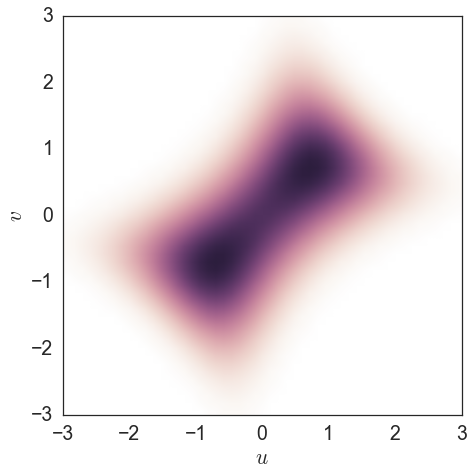
\includegraphics[width=\textwidth]{signflip_bayes_posterior}
\caption{True posterior $p(u, v | r)$ has signflip symmetry.}
\end{subfigure}
\begin{subfigure}[t]{.3\textwidth}
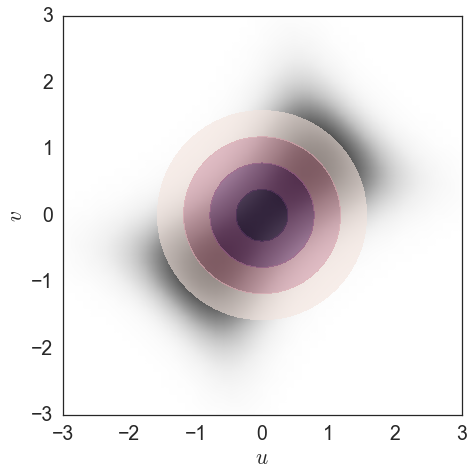
\includegraphics[width=\textwidth]{signflip_mfvb_posterior}
\caption{Mean-field Gaussian approximation.}
\end{subfigure}
\begin{subfigure}[t]{.3\textwidth}
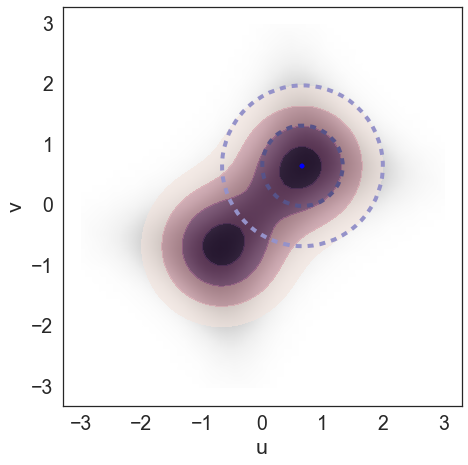
\includegraphics[width=\textwidth]{signflip_symmetric_posterior}
\caption{Symmetrized approximation $\tilde{q}$ mixing $q^*(u,v)$ (dotted) and $q^*(-u,-v)$.}
\end{subfigure}
\caption{Implicit regularization in the scalar factorization model $r = uv +
  \epsilon$; $u,v \in \mathbb{R}$, given observed
  $r=1.5$. The mean field approximation finds a degenerate mode at the
origin, while the symmetrized $\tilde{q}$ captures both true modes.}
\label{fig:signflip_demo}
\end{figure}

\begin{figure}[t]
\centering
\begin{subfigure}[t]{.3\textwidth}
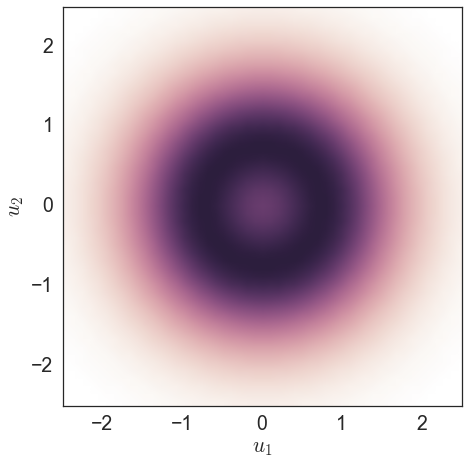
\includegraphics[width=\textwidth]{rot_bayes_posterior}
\caption{True posterior $p(\v{u} | r)$ has rotational symmetry.}
\end{subfigure}
\begin{subfigure}[t]{.3\textwidth}
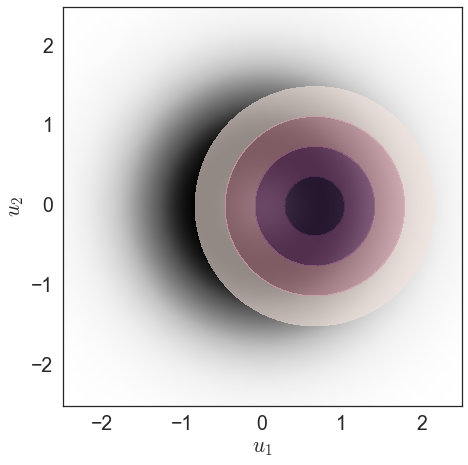
\includegraphics[width=\textwidth]{rot_mfvb_posterior}
\caption{Mean-field Gaussian approximation is pulled towards the origin.}
\end{subfigure}
\begin{subfigure}[t]{.3\textwidth}
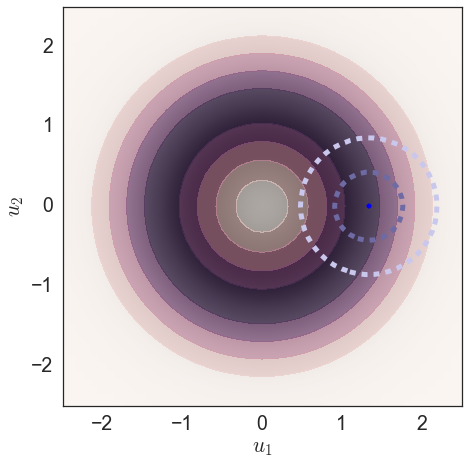
\includegraphics[width=\textwidth]{rot_symmetric_posterior}
\caption{Symmetrized approximation $\tilde{q}$ formed by rotation
  of base Gaussian $q^*$ (dotted).}
\end{subfigure}
\caption{Implicit regularization of the marginal posterior $p(\v{u} | r)$ in the
  overparameterized scalar model $r = \v{u}\v{v}^T + \epsilon$;
  $\v{u},\v{v} \in \mathbb{R}^{1 \times 2}$, given observed
  $r=2$. This rotational symmetry is a special case of the more general
  symmetry in the joint column space of $\v{U}$ and $\v{V}$.}
\label{fig:rot_demo}
\vspace{-1.3em}
\end{figure}

\begin{figure}
\centering
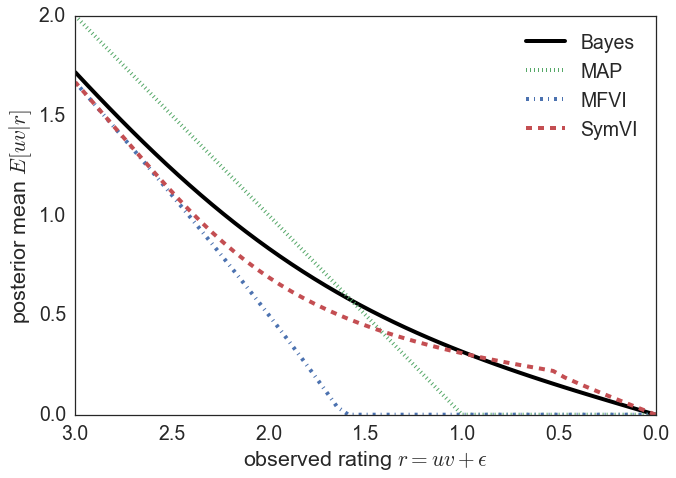
\includegraphics[width=0.5\textwidth]{signflip_sv_plot}
\caption{Predictive mean $\E[uv | r]$ in the scalar factorization model $r = uv + \epsilon$, with $u,
  v, \epsilon \sim \N(0, 1)$. Standard mean field (MFVI)
  and even MAP are subject to degenerate solutions at zero for small $r$, while
  inference with a symmetrized posterior invariant to signflips (SymVI)
  more closely recovers the Bayes predictive mean.}
\label{fig:signflip_svs}
\end{figure}

We consider probability models of the form $p(\v{x}, \v{z})$ where $\v{x}$ and
$\v{z}$ are observed and latent variables, and perform
inference by minimizing the exclusive divergence $KL[q \| p]$
between an approximate posterior $q_{\v{\theta}}(\v{z})$ and the true
posterior $p(\v{z}|\v{x})$. This is equivalent to maximizing a lower
bound on the log model evidence,
\begin{equation}
\mathcal{L}(\v{\theta})\label{eqn:elbo} = \E_{\v{z}\sim q_\theta}\left[\log p(\v{x}, \v{z}) -
                \log q_\theta(\v{z})\right] \le \log p(\v{x}) 
\end{equation}
known as the Evidence Lower Bound or \elbo \; \citep{bishop2006pattern}. 
The so-called reparameterization trick enables practical inference via
gradient-based stochastic optimization of $\mathcal{L}(\v{\theta})$, as
long as the sampling process $\v{z}\sim q_\theta$ can be expressed as
a differentiable transformation $\v{z} = f_\theta(\v{\epsilon})$ of a random
source $\v{\epsilon}$. \citep{kingma2013auto, kucukelbir2016automatic}. 

We are interested in cases where the model density in the latent space is invariant under
the action of transformations from a group $\G$, so that 
$p(\v{x}, \v{z}) = p(\v{x}, \v{T}\v{z}) \;\; \forall \; \v{T} \in
\G.$
We propose to exploit this structure by imposing the same invariance
on our variational posterior. 

We define a {\em symmetrized
  posterior} $\tilde{q}_{\theta}$ by a two-step sampling
process: first sample $\v{z}^*$ from some base posterior $q_\theta^*$, then apply a random
transformation $\v{T}$ to generate $\v{z} =
\v{T}\v{z}^*$. Equivalently we can write $\tilde{q}_{\theta}$ as an
explicit mixture with respect to the uniform (Haar) measure on $\G$,
given by
\begin{align}
\tilde{q}_{\theta}(\v{z}) &= \int_{\v{T}\in \G}
                            q^*_{\theta}(\v{T}^{-1}\v{z})
                            \left|\v{T}^{-1}\right|dV(\v{T})
\end{align}
where $\left|\v{T}^{-1}\right|$ is the Jacobian
determinant (unity for orthogonal transformations). It is clear that this
respects the symmetry $\tilde{q}_\theta(\v{z})
=\tilde{q}_\theta(\v{T}\v{z})$ for all $\v{T}\in\G$. 

Plugging $\tilde{q}_\theta$ into the \elbo, we note that
expectations under $\tilde{q}_\theta$ can be written as a nested expectation
over a base sample $\v{z}^*$ and transformation $\v{T}$:
\begin{align*}
\mathcal{L}(\tilde{q}_\theta) &= \E_{\v{z}\sim \tilde{q}_\theta}\left[\log p(\v{x}, \v{z}) - \log \tilde{q}_\theta(\v{z})\right]\\
&= \E_{\v{z}^*\sim q^*_\theta}\left[\E_\v{T}\left[\log p(\v{x}, \v{T}\v{z}^*) -
  \log \tilde{q}_\theta(\v{T}\v{z}^*)\right]\right]
\end{align*}
Since the model density $p$ is invariant to $\v{T}$ by assumption, and
the symmetrized posterior $\tilde{q}_\theta$ is also
invariant by construction, the expectation over $\v{T}$ is vacuous. Dropping it yields the
final objective
\begin{align}
\mathcal{L}(\tilde{q}_\theta) &= \E_{\v{z}^*\sim q^*_\theta}\left[\log p(\v{x}, \v{z}^*) - \log \tilde{q}_\theta(\v{z}^*)\right]\label{eqn:symmetrized_elbo},
\end{align}
which differs from (\ref{eqn:elbo}) only in that we are now
evaluating the mixture density $\log \tilde{q}_\theta$ in place of the
original $\log q_\theta$. In particular, the expectation is
only under the base posterior, so reparameterization
gradients present no special difficulty, and we are still free to
exploit any analytic structure in the expected log density $\E_{\v{z}^*\sim q^*_\theta}\left[\log p(\v{x}, \v{z}^*)\right]$. 

\subsection{Signflip symmetry}

The framework described above is applicable generally to any base
family $q^*_\theta$ and symmetry group $\G$; the challenge in practice is to efficiently
compute or bound the mixture entropy $\mathcal{H}(\tilde{q}_\theta) =
\E[-\log \tilde{q}_\theta(\v{z}^*)]$. Under a Monte Carlo approximation this
reduces to computing the log density $-\log \tilde{q}_\theta(\v{z}^*)$
at values $\v{z}^*$ sampled from the base posterior. In the simple case of signflip
symmetries, this can be done tractably with an explicit sum $\log
\tilde{q}(\v{z}) = \log \frac{1}{2}\left(q(\v{z}) + q(-\v{z})\right)$.

Signflip symmetries arise in the special case of matrix
factorization where all quantities are scalar
(\Cref{fig:signflip_demo}). In this case it is also tractable to
numerically compute the Bayes predictive mean. \Cref{fig:signflip_svs}
compares predictive means as a function of the observed scalar value $r$, showing
that while standard methods exhibit degenerate regularization,
predictions using the symmetrized posterior track the true Bayes
prediction much more closely. 

% TODO in full version mention combinatorial signflip symmetry, permutation symmetry 

\subsection{General orthogonal symmetry}
\begin{figure}[t]
\centering
\begin{subfigure}[t]{.5\textwidth}
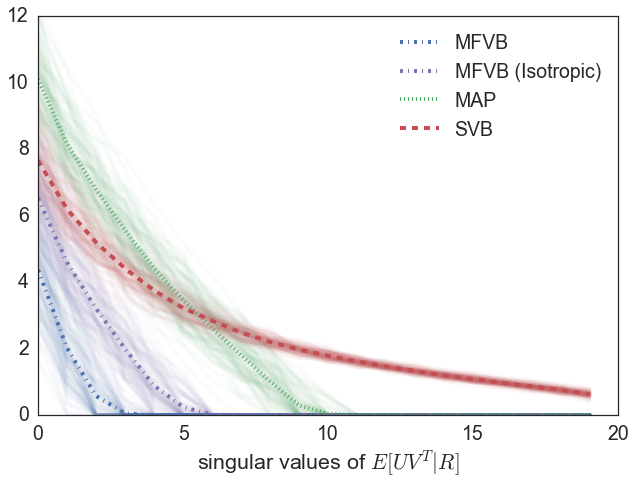
\includegraphics[width=\textwidth]{rot_sv_plot}
\caption{Singular values of predictive mean $\E[\v{U}\v{V}^T |
  \v{R}]$. }
\label{fig:rot_svs}
\end{subfigure}
\begin{subfigure}[t]{.45\textwidth}
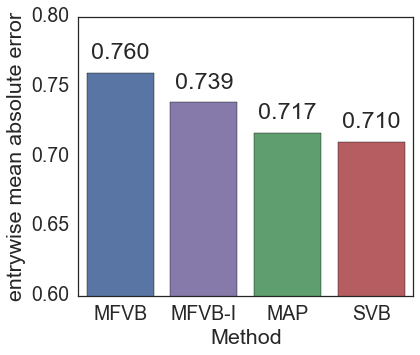
\includegraphics[width=\textwidth]{rot_error_barplot}
\caption{Mean absolute entrywise reconstruction error $\|\E[\v{U}\v{V}^T | \v{R}] - \v{U}\v{V}^T
  \|_1$.}
\label{fig:rot_error}
\end{subfigure}
\caption{Inference on 80 synthetic samples with $n=m=40$, $k=20$, and $\sigma_n
  = 2$. Orthogonally symmetrized VI (SymVI) uses the full capacity of
  latent traits, resulting in better predictions.}
\end{figure}

\vspace{-0.5em}
Our main technical contribution is an efficient approximation to the continuous mixture density
\begin{align*}
\log \tilde{q}(\v{X}) &= \log \int_{\v{T}\in \O(k)} \N(\v{X}; \v{M}\v{T}, \v{T}^T\v{\Sigma} \v{T}) dV(\v{T})
\end{align*}
in which an elementwise matrix Gaussian $q(\v{X})=\N(\v{X}; \v{M}, \v{\Sigma})$ is
integrated over the orthogonal group $\O(k)$. For space considerations
we defer details to \Cref{sec:rot_density}. Our current analysis assumes an isotropic covariance ($\v{\Sigma}=c\I$)
which we hope to relax in future work. 

Informally, any rotation $\v{T}$ acting within the nullspace of $\v{M}$
generates a mixture component $\v{M}\v{T}=\v{M}$ equivalent to the base distribution;
such rotations are ``wasted'' in the sense that they do not increase
the mixture entropy $\mathcal{H}(\tilde{q})$ relative to the base
$\mathcal{H}(q)$. Inference using the mixture entropy $\mathcal{H}(\tilde{q})$
therefore penalizes the nullspace dimension of the posterior mean, avoiding component collapse by encouraging nonzero singular values. This effect is seen in \Cref{fig:rot_svs}, which plots
singular values of the predictive mean $\E[\v{U}\v{V}^T | \v{R}]$ from a relatively noisy
($\sigma_n=2$) synthetic 20-trait model. While the mean field VI and MAP
solutions (and MFVI with isotropic covariance, included
for comparison) shrink many traits to zero, symmetrized VI uses
the model's full capacity. \Cref{fig:rot_error} shows that this is
reflected in predictive performance: symmetrized VI yields better
reconstructions of the true
generative ratings $\v{U}\v{V}^T$ than the implicitly-regularized MAP
and (especially) mean field estimates. 

\section{Future work}
\vspace{-0.5em}
These preliminary results demonstrate that explicitly accounting for
parameter symmetries can yield better inferences. In future work we
hope to consider symmetrization of non-isotropic Gaussians and
more flexible approximating classes
\citep{salimans2015markov,rezende2015variational,tran2016variational},
as well as permutation, translation, and scaling symmetries. We are
especially interested in the use of symmetrized posteriors for
automatic relevance determination (ARD) and model selection,
as well as extensions to stochastic inference in ``deep'' models
such as variational autoencoders.

%evaluating predictive variance. 
\newpage
\bibliographystyle{apa}
\bibliography{references}

\appendix 
\section{Orthogonal Gaussian mixture densities}
\label{sec:rot_density}

We consider as a base density the elementwise (mean-field) Gaussian
\[q^*(\v{X}) = \N\left(\v{X}; \v{M},  \v{S}\right)  = \prod_{i=1}^{n+m} \prod_{j=1}^k \N(x_{ij}; m_{ij}, s_{ij})\]
in which we let $\v{M}, \v{S}$ contain elementwise means and variances respectively for a
matrix-valued variable $\v{X}$; in matrix
factorization we will let $\v{X}= \left[\begin{array}{l}\v{U}\\\v{V}\end{array}\right] \in \mathbb{R}^{(n+m)\times k}$ be the stacked matrix of
latent traits. We will focus on the restrictive case where each row is described by the
same diagonal covariance $\v{\Sigma} \in \mathbb{R}^{k \times k}$, so that the density can be written
\[q^*(\v{X}) \propto \exp\left\{-\frac{1}{2}\Tr\left[(\v{X}-\v{M})\v{\Sigma}^{-1}(\v{X}-\v{M})^T\right]\right\};\]
 below we will restrict this further to the case where $\v{\Sigma} = c\I$
 is isotropic. We hope to relax both of these assumptions in future work. 

We consider the symmetrized approximate posterior
\begin{align*}
\tilde{q}(\v{X}) = \int_{\v{T}\in \O(k)} \N(\v{X}\v{T}^T; \v{M}, \v{\Sigma}) dV(\v{T}) = \int_{\v{T}\in \O(k)} \N(\v{X}; \v{M}\v{T}, \v{T}^T \v{\Sigma} \v{T}) dV(\v{T})
\end{align*}
which is a continuous mixture of Gaussians with means and (co)variances
corresponding to rotations within the column space of $\v{M}$. The log
density decomposes into that of the base density $q$, plus a correction term $r(\v{X}, \v{M}, \v{\Sigma})$:
\begin{align}
\log \tilde{q}(\v{X}) &= \log \int_{\v{T}\in \O(k)} \N(\v{X}\v{T}^T; \v{M}, \v{\Sigma}) dV(\v{T})\nonumber\\
&=\log \N(\v{X}; \v{M}, \v{\Sigma}) + \log \int_{\v{T}\in \O(k)} \frac{\N(\v{X}\v{T}^T; \v{M}, \v{\Sigma})}{\N(\v{X}; \v{M}, \v{\Sigma} ) }  dV(\v{T})\nonumber\\
&=\log q^*(\v{X}) + r(\v{X}, \v{M}, \v{\Sigma})\label{eqn:symmetrized_orthog}
\end{align}
Intuitively the correction $r$ captures the rotational asymmetry of the
base distribution $q$: if $q$ is already rotationally symmetric (e.g.,
if $\v{M}=\v{0}$, so $q$ is centered at the origin)
then the ratio inside the integral is unity and the correction is zero. Examining this correction more closely,
\begin{align*}
r(\v{X}, \v{M}, \v{\Sigma}) &= \log \int_{\v{T}\in \O(k)} \frac{\N(\v{X}\v{T}^T; \v{M}, \v{\Sigma})}{\N(\v{X}; \v{M}, \v{\Sigma} ) }  dV(\v{T})\\
&= \log \int_{\v{T}\in \O(k)} e^{-\frac{1}{2} \Tr \left[
  (\v{X}\v{T}^T-\v{M})\v{\Sigma}^{-1}(\v{X}\v{T}^T-\v{M})^T \right] + \frac{1}{2}\Tr \left[
  (\v{X}-\v{M})\v{\Sigma}^{-1}(\v{X}-\v{M})^T \right] }  dV(\v{T})\\
&= \log \int_{\v{T}\in \O(k)} e^{-\frac{1}{2} \left( \Tr \left[\v{X}\v{T}^T\v{\Sigma}^{-1}\v{T}\v{X}^T\right] - \Tr\left[\v{X}\v{\Sigma}^{-1}\v{X}^T\right]\right)}
  e^{\Tr\left[\v{X}\v{T}^T\v{\Sigma}^{-1}\v{M}^T \right] - \Tr\left[\v{X}\v{\Sigma}^{-1}\v{M}^T\right]} dV(\v{T})\\
&= \log \int_{\v{T}\in \O(k)} f(\v{T}) g(\v{T}) dV(\v{T})
\end{align*}
we find that it is effectively an inner product of two functions $f,g$
over the orthogonal group. The first factor, $f(\v{T}) = \exp\left\{-\frac{1}{2}
  \left( \Tr \left[\v{X}\v{T}^T\v{\Sigma}^{-1}\v{T}\v{X}^T\right] -
    \Tr\left[\v{X}\v{\Sigma}^{-1}\v{X}^T\right]\right)\right\},$
measures the discrepancy between the precision matrix $\v{\Sigma}^{-1}$ and its
transformed counterpart $\v{T}\v{\Sigma}^{-1}\v{T}^T$, while the second factor, $g(\v{T}) = \exp\left\{\Tr\left[\v{X}\v{T}^T\v{\Sigma}^{-1}\v{M}^T \right] -
  \Tr\left[\v{X}\v{\Sigma}^{-1}\v{M}^T\right]\right\},$ measures the extent to which a
given transformation $\v{T}$ aligns the observed value $\v{X}$ with the mean
$\v{M}$. Note that $f$ vanishes in the case of isotropic covariance $\v{\Sigma} = c\I$, since this implies
$\v{T}^T\v{\Sigma}^{-1}\v{T} = \v{\Sigma}^{-1}$. In this case we have
\begin{align*}
r(\v{X}, \v{M}, \v{\Sigma}) &= \log \int_{\v{T}\in \O(k)}  g(\v{T}) dV(\v{T})\\
&= \log \int_{\v{T}\in \O(k)}  \exp\left\{\Tr\left[c^{-1} \v{M}^T\v{X}\v{T}^T \right] -
  \Tr\left[c^{-1}\v{M}^T \v{X}\right]\right\} dV(\v{T}),
\end{align*}
and letting $\v{A} = c^{-1}\v{M}^T \v{X}$, this simplifies to
\begin{align*}
&= \log \int_{\v{T}\in \O(k)}  \exp\left\{\Tr\left[\v{A}\v{T}^T \right] - \Tr\left[\v{A}\right]\right\} dV(\v{T})\\
&= - \Tr\left[\v{A}\right] + \log \pFq{0}{1}\left[\frac{k}{2}; \frac{1}{4}\v{A}\v{A}^T\right]
\end{align*}
where the hypergeometric function $\pFq{0}{1}\left[\frac{k}{2}; \frac{1}{4}\v{A}\v{A}^T\right] = \int_{\v{T}\in \O(k)}  \exp\left\{\Tr\left[\v{A}\v{T}^T \right]\right\}
  dV(\v{T})$ is a form of matrix-argument Bessel function
  \citep{herz1955bessel}, also
  arising in the analysis of the non-central Wishart distribution
  \citep{muirhead1982aspects}. Notably it depends on $\v{A}$ only
  through its singular values $(\sigma_i)_{i=1}^k$. This conforms with
  the intuition, stated above, that the effect of inference with an orthogonal
  mixture of Gaussians should be to encourage nonzero singular values
  in $\v{M}$ (and, by extension, $\v{A}$). 

\citet{butler2003laplace} derive a Laplace approximation to $\pFq{0}{1}$,
given by
\begin{align}
\pFq{0}{1}\left[\frac{k}{2}; \frac{1}{4}\v{A}\v{A}^T\right] \approx
  \frac{\prod_{i=1}^k (1-\hat{y}_i^2)^{k/2}e^{\sigma_i\hat{y}_i}}
  {\sqrt{\prod_{i=1}^k\prod_{j=1}^k (1-\hat{y}_i^2 \hat{y}_j^2)}}\label{eqn:laplace}
\end{align}
for $\hat{y}_i = 2\sigma_i/(k \sqrt{4\sigma_i^2 / k^2 + 1} +
1)$; in their evaluations this approximation demonstrates ``very high
accuracy in a variety of settings''. It can be implemented stably in the log domain as a differentiable
function of the singular values $\sigma$. 

We use use the Laplace approximation
(\ref{eqn:laplace}) to implement the symmetrized density
(\ref{eqn:symmetrized_orthog}), with automatic gradients computed
using TensorFlow. 
Code is given in \Cref{listing:stuff}. Although TensorFlow does not
implement gradients for the SVD
operator $\v{A} = \v{U} \diag(\sigma) \v{V}^T$, 
we exploit the fact that $\v{U}\diag(\sigma) = \v{A}\v{V}$, allowing us to
approximate gradients $\frac{\partial
  \sigma(\v{A}) }{\partial \v{A}}$ by differentiating through the
column norms of $\v{A}\v{V}$ holding fixed the singular vectors
$\v{V}$. Note that $\v{A}$ is a $k \times k$ matrix, where the trait
dimension $k \ll n, m$ does not depend on the data size, so computing the SVD on each
gradient update is relatively cheap. In practice we do not observe
significant slowdowns from inference under the symmetrized $\tilde{q}$
relative to the base posterior $q^*$.

\begin{listing}
\begin{minted}{python}

def symmetrized_log_density(X, M, c):
    # X, M: 2D Tensors of matching dimensions
    # c: scalar (isotropic) variance
    
    log_q = gaussian_log_density(X, M, c)

    # correction term r depends on singular vals of X'M
    A = tf.matmul(tf.transpose(X), M) / c
    svs = differentiable_singular_vals(A)
    r = log_bessel(svs, k) - tf.trace(A)
    return log_q + r

def gaussian_log_density(X, M, c):
    Z = tf.square(X-M) / c
    lps = -0.5 * Z   - .5 * tf.log(2*np.pi * tf.ones_like(X) * c)
    return tf.reduce_sum(lps)

def differentiable_singular_vals(A):
    # returns singular vals of A with approximate gradients. 
    d, u, v = tf.svd(A)
    ud = tf.matmul(A, tf.stop_gradient(v))
    return tf.sqrt(tf.reduce_sum(tf.square(ud), 0))

def log_bessel(svs, n):
    def r(u):
          return u/(tf.sqrt(tf.square(u) + 1.0) + 1.0)
    ys = r(2.0*svs / n)
    y2 = tf.square(ys)
    y2r = tf.reshape(y2, (n, 1))
    y2pairs = tf.matmul( y2r, tf.transpose(y2r))
    log_denom = .5 * tf.reduce_sum(tf.log(1-y2pairs))
    log_num = tf.reduce_sum(svs*ys + n/2.0 * tf.log((1-y2)))
    return log_num - log_denom

\end{minted}
\caption{TensorFlow implementation of orthogonally symmetrized
  Gaussian log density.}
\label{listing:stuff}
\end{listing}

\end{document}

%%% Local Variables:
%%% LaTeX-command: "latex -shell-escape"
%%% End: